\documentclass[11pt]{article}

\usepackage{float}
\usepackage{hyperref}
\usepackage{graphicx}
% formatting
\usepackage{verbatim}
\usepackage{moreverb}
\usepackage{minted}
\usepackage{parskip}
\usepackage{amsmath}
\usepackage[listings]{tcolorbox}
\usepackage{enumerate}
\let\verbatiminput=\verbatimtabinput
\def\verbatimtabsize{4\relax}

\newcommand{\RepoRootPath}{fpga\_labs\_sp21}

\tcbset{
texexp/.style={colframe=black, colback=lightgray!15,
         coltitle=white,
         fonttitle=\small\sffamily\bfseries, fontupper=\small, fontlower=\small},
     example/.style 2 args={texexp,
title={Question \thetcbcounter: #1},label={#2}},
}

\newtcolorbox{texexp}[1]{texexp}
\newtcolorbox[auto counter]{texexptitled}[3][]{%
example={#2}{#3},#1}

\setlength{\topmargin}{-0.5in}
\setlength{\textheight}{9in}
\setlength{\oddsidemargin}{0in}
\setlength{\evensidemargin}{0in}
\setlength{\textwidth}{6.5in}

% Useful macros

\newcommand{\note}[1]{{\bf [ NOTE: #1 ]}}
\newcommand{\fixme}[1]{{\bf [ FIXME: #1 ]}}
\newcommand{\wunits}[2]{\mbox{#1\,#2}}
\newcommand{\um}{\mbox{$\mu$m}}
\newcommand{\xum}[1]{\wunits{#1}{\um}}
\newcommand{\by}[2]{\mbox{#1$\times$#2}}
\newcommand{\byby}[3]{\mbox{#1$\times$#2$\times$#3}}


\newenvironment{tightlist}
{\begin{itemize}
 \setlength{\parsep}{0pt}
 \setlength{\itemsep}{-2pt}}
{\end{itemize}}

\newenvironment{titledtightlist}[1]
{\noindent
 ~~\textbf{#1}
 \begin{itemize}
 \setlength{\parsep}{0pt}
 \setlength{\itemsep}{-2pt}}
{\end{itemize}}

% Change spacing before and after section headers

\makeatletter
\renewcommand{\section}
{\@startsection {section}{1}{0pt}
 {-2ex}
 {1ex}
 {\bfseries\Large}}
\makeatother

\makeatletter
\renewcommand{\subsection}
{\@startsection {subsection}{1}{0pt}
 {-1ex}
 {0.5ex}
 {\bfseries\normalsize}}
\makeatother

% Reduce likelihood of a single line at the top/bottom of page

\clubpenalty=2000
\widowpenalty=2000

% Other commands and parameters

\pagestyle{myheadings}
\setlength{\parindent}{0in}
\setlength{\parskip}{10pt}

% Commands for register format figures.

\newcommand{\instbit}[1]{\mbox{\scriptsize #1}}
\newcommand{\instbitrange}[2]{\instbit{#1} \hfill \instbit{#2}}

\begin{document}

\def\PYZsq{\textquotesingle}
\title{\vspace{-0.4in}\Large \bf EECS 151/251A FPGA Spring 2021\\
Lab 2:\\Sequential Circuits, Simulation, Button Parser\vspace{-0.1in}}

\author{Prof. John Wawrzynek \\
TAs: Sean Huang, Tan Nguyen \\ Department of Electrical Engineering and Computer Sciences\\
College of Engineering, University of California, Berkeley}
\date{}
\maketitle

\newcommand{\headertext}{EECS 151/251A FPGA Lab 2: Simulation and Sequential Circuits}
\markboth{\headertext}{\headertext}
\thispagestyle{empty}

\section{Before You Start This Lab}\label{sec:begin}
Run \verb|git pull| in \verb|fpga_labs_sp21|.

Before you begin this lab, please review our lecture and discussion slides on Verilog. Another useful resource is \href{http://inst.eecs.berkeley.edu/~eecs151/fa19/files/verilog/Verilog_Primer_Slides.pdf}{Verilog Primer Slides}. You should understand some fundamental concepts of hardware design in Verilog, such as combinational logic and sequential logic, in order to complete this lab. We also suggest that you take some time to look through these documents that will help you better understand some Verilog constructs.

\begin{enumerate}
  \item \href{http://inst.eecs.berkeley.edu/~eecs151/sp21/files/verilog/wire_vs_reg.pdf}{\color{blue}{wire\_vs\_reg.pdf}} - The differences between wire and reg nets and when to use each of them.
  \item \href{http://inst.eecs.berkeley.edu/~eecs151/sp21/files/verilog/always_at_blocks.pdf}{\color{blue}{always\_at\_blocks.pdf}} - Understanding the differences between the two types of always @ blocks and what they synthesize to.
\end{enumerate}

Also, please note that we adopt the "No register inference" policy in this semester (refer to slide 18, Lec 4). Therefore, you should not write any sequential always blocks in your code. You should not need to use non-blocking assignments or \textit{reg} nets for registers. Instead, \textbf{please instantiate a REGISTER* module from the lib/EECS151.v file from our lab Github repository whenever you want to declare a register}. This only applies to Verilog design file, but not necessarily to testbench code as we will see later.

The previous lab walked you through how to create and manage an FPGA project in Vivado Design suite. In this lab, we cover Simulation using Vivado Design suite. The first few labs are meant to be long and tedious. Don't be intimidated! As you will see, being a good hardware designer does not mean just writing Verilog or any HDL code; you also need to have a firm understanding on the design tools to productively generate a working hardware implementation for your FPGA.

We also learn how to design a \href{http://www.labbookpages.co.uk/electronics/debounce.html}{\underline{Debouncer Circuit}} which can reliably sample button presses to provide control signals for our sequential digital circuits. Read the ``What is Switch Bounce'' section about why we need a debouncer circuit. Read the ``Digital Switch Debouncing'' section about the implementation of a debouncer circuit.

\section{Structural coding vs. Behavioral coding}

In this section, you will design a 3-bit adder using either structural or behavioral approach in Verilog.

\subsection{Build a Structural 3-bit Adder}
What do we mean by "structural approach"? It builds a circuit using only Boolean logic gates and multiplexers.
It's similar to how you are drawing your design in a schematic editor, but we use Verilog instead.
To help you with this task, please refer to the `Code Generation with for-generate loops' slide in the Verilog Primer Slides (slide 35).

\begin{enumerate}
  \item Create a new project (or reuse existing project). Add the following Verilog files to your project: \verb|lab2/src/full_adder.v|, \verb|lab2/src/structural_adder.v|, \verb|lab2/src/z1top_adder.v|. Also add the constraint file to your project: \verb|lab2/consrr/z1top.xdc|. For your own convenience, the pin assigments for the buttons, switches, and LEDs have been done. Notice their relevance to the top-level Verilog module \texttt{z1top\_adder}.
  \item Open \verb|full_adder.v|; fill in the logic to produce the full one-bit adder outputs from the inputs.
  \item Open \verb|structural_adder.v| and construct a ripple carry 3-bit adder using the full one-bit adder cells you designed earlier. Use `for-generate loop' construct to make your code compact.
  \item Finally, inspect the \verb|z1top_adder.v| top-level module and see how your structural adder is instantiated and hooked up to the top-level signals. For now, just look at the \verb|user_adder| instance of your structural adder. Note how the adder operands and result are constructed from the input/output signals of the top-level Verilog module, and in turn the buttons and switches and LEDs on the FPGA.
  \item Set \verb|z1top_adder.v| as the top-level module by right-clicking \texttt{z1top\_adder} in Sources $\rightarrow$ Design Sources and click `Set as Top'. You can skip this step if it is already the top-level module.
  \item Run bitstream generation as usual.
  \item Program the FPGA and test out the design. Try different combinations of buttons and switches. Make sure you get correct results from your adder via the LEDs.
\end{enumerate}

\subsection{Inspection of Structural Adder}
\subsubsection{Schematics and FPGA Layout}
Take a look at how the Verilog you wrote mapped to the primitive components on the FPGA.
Three levels of schematic are generated for you once you've run the pipeline.
In the \emph{Flow Navigator}, you can view \emph{Schematic}s under

\begin{enumerate}
  \item \emph{RTL Analysis} $\rightarrow$ \emph{Open Elaborated Design}
  \item \emph{Synthesis} $\rightarrow$ \emph{Open Synthesized Design}
  \item \emph{Implementation} $\rightarrow$ \emph{Open Implemented Design}
\end{enumerate}

The first two will give you a fairly straightforward hierarchical block-level view of your design. You will find your circuit by drilling down into the \verb|user_adder| module (that's the name you gave the instantiation of \verb|structural_adder| in \verb|z1top_adder.v|).
Check to see that your structural adder module is hooked up properly and looks sane.
It's ok if the wires don't appear to be connected, just hover your mouse over the endpoints on the schematic and ensure that the connections are as you expect.
Take note of the primitive blocks used in your circuit.

In the RTL Analysis (1) you are viewing a visualization of the topology your RTL describes. At this point, logic elaboration is very abstract: you'll notice that your logic is expressed in terms of the logic gates you described (XOR, AND, etc). Any logic you describe in RTL is included, even if it's disconnected. In the Synthesis schematic (2) this logic has been elaborated further into what look like FPGA elements, but still at higher layer of abstraction, and with some unused signals still present. In the final schematic of the three, Implementation (3), the schematic now shows which of the elements in your nominated chip are actually targeted. Superfluous logic has been elided from the design.

Finally, you also look at how your circuit was placed and laid out on the FPGA. Once you've run the pipeline, open \emph{Implemented Design}, click on the \emph{Window} menu, and select \emph{Device}. You'll be presented with a layout of the FPGA package as in box 1 in the figure below. It'll be hard to see with a small design, but the logic elements you've ended up using with your design will be highlighted. You can highlight your own nets in the diagram to make it easier to find them by selecting a net or signal from the Netlist pane (\emph{Window} $\rightarrow$ \emph{Netlist}; see box 2).

\begin{center}
  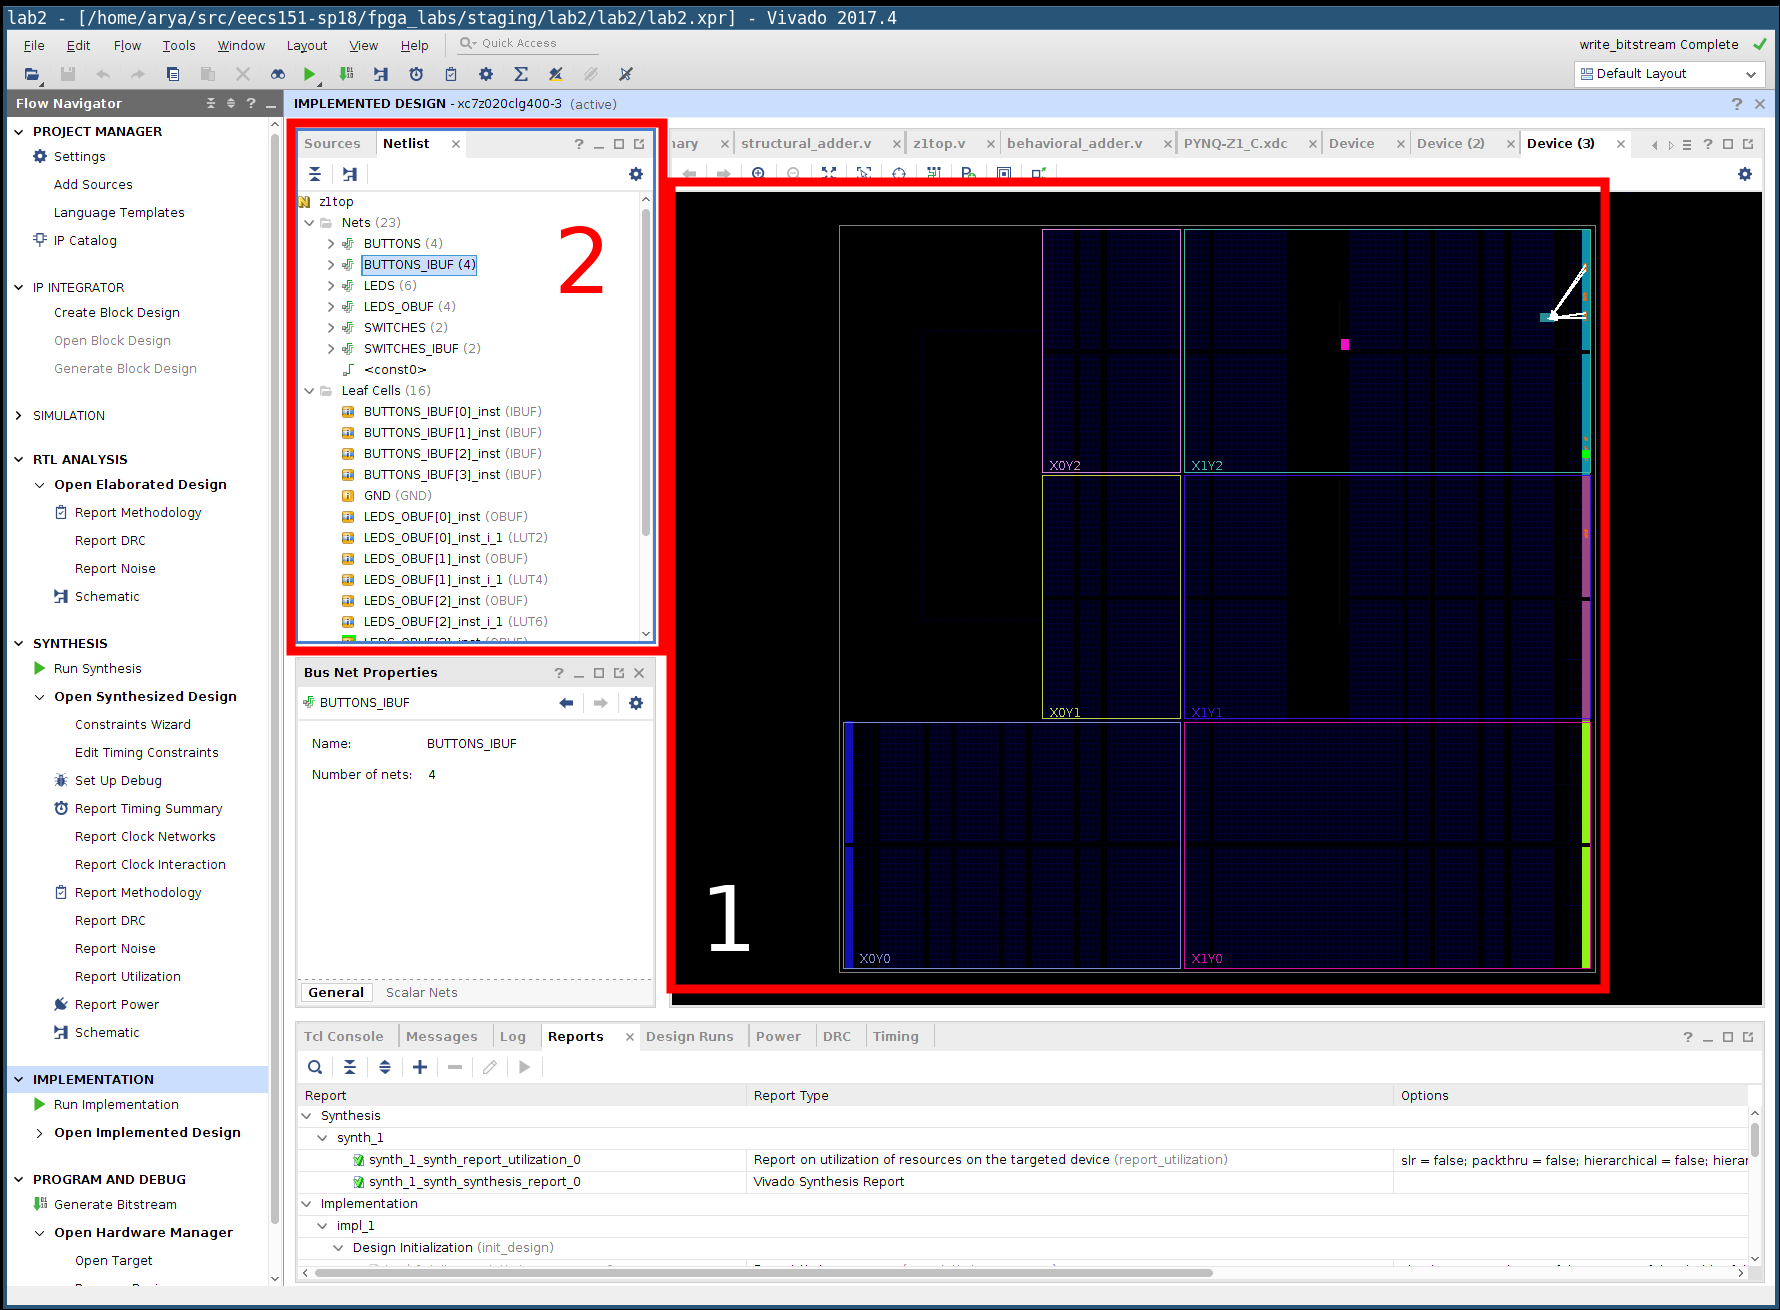
\includegraphics[width=0.7\textwidth]{figs/fpga_layout.png}
\end{center}

Explore your design and look for the modules that you wrote. If you scroll down in the \verb|Netlist Window| you should see various components of your logic. Some elements are mapped to LUTs: somewhere buried in their properties is the type of slice. See if you can find out which nets have been assigned to LUTs, and how they are connected. Go ahead and explore several SLICELs that implement the structural adder to see how they are connected to each other and the outputs of your circuit.

\subsection{Build a Behavioral 3-bit Adder}

Check out \verb|behavioral_adder.v|. It has already been filled with the appropriate logic for you. Notice how behavioral Verilog allows you to describe the function of a circuit rather than the topology or implementation. Modify your top-level module in \verb|z1top_adder.v| to use the behavioral adder instead of the structural adder. Generate and load the bitstream to the FPGA. Verify if the behavioral adder works correctly.

Behavioral coding style allows designers to build their designs using arithmetic operators, comparators, or software-like constructs such as \verb|if-else|, \verb|case| statements (to generate muxes), which greatly improves productivity.

\subsection{Inspection of Behavioral Adder Schematics and FPGA Layout}
Go through the same steps as you did for inspecting the structural adder. View the schematics at successive levels of logic elaboration and how FPGA components are connected.

\subsection{Questions}\label{sec:Q1}
\begin{enumerate}
 \item Record and note down any differences you see between both types of adders in the schematics and the FPGA layouts (from \emph{RTL Elaborated Design} to \emph{Implemented Design}).
\end{enumerate}

\section{Build Your First Sequential Digital Circuit}

In this section, you will design a 4-bit wrap-around counter that increments every one second. The counter value is shown on the LEDS 0-3 of the PYNQ board.

\subsection{Clock Sources}
Look at the \href{https://reference.digilentinc.com/reference/programmable-logic/pynq-z1/reference-manual}{\color{blue}{PYNQ Reference Manual}}.
Read Section 11 about the clock sources available on the PYNQ.
We are using the 125 MHz clock from the Ethernet PHY IC on the PYNQ board that connects to pin H16 of the FPGA chip.

Look at the \verb|lab2/src/z1top_counter.v| top-level module and its \verb|CLK_125MHZ_FPGA| input.
\begin{minted}{verilog}
module z1top_counter (
    input CLK_125MHZ_FPGA,
    ...
);
\end{minted}

We can access the clock signal from our Verilog top-level module and can propagate this clock signal to any submodules that may need it.

Next, open the constraint file \verb|lab2/constr/z1top.xdc|, \textbf{add the following TCL commands to it}

\begin{minted}[fontsize=\small]{tcl}
set_property -dict { PACKAGE_PIN H16 IOSTANDARD LVCMOS33 } [get_ports { CLK_125MHZ_FPGA }];
create_clock -add -name CLK_125MHZ_FPGA -period 8.00 -waveform {0 4} [get_ports { CLK_125MHZ_FPGA }];
\end{minted}

The first command assigns our clock input signal to H16, just as specified in the PYNQ-Z1 Reference Manual. The second command informs Vivado that our input clock signal has a period of 8 ns (125 MHz) which matches the actual clock frequency from pin H16. This is the target clock constraint (or often referred as frequency constraint) of your design. Vivado will try to optimize your design to meet this constraint, and the post-routing timing analysis will report whether it is the case. Please do not forget to set a clock constraint when you design a sequential circuit.

\subsection{Build a 4-bit Counter}

Your circuit receives an input clock signal with a clock period of 8 ns (125 MHz). How many cycles of this clock signal are equivalent to one second? Note that
\begin{align*}
Time (sec) = Clock\ Period \times Number\ of\ cycles
\end{align*}
You will need to wait for this amount of clock cycles before incrementing your LED counter. You may use an additional counter to keep track of this.

You are required to use the library of registers that we provide you (\verb|lib/EECS151.v|). Please instantiate a REGISTER* module whenever you want to build a register. Please do \emph{not} write any sequential always block (e.g., \texttt{always @(posedge clock)}) or non-blocking assignment in your code.

\begin{enumerate}
  \item Create a new project (or reuse existing project). Add the following Verilog file to your project: \verb|lab2/src/z1top_counter.v|.
  \item Add the EECS151 library of registers to your project \verb|lib/EECS151.v|.
  \item Open \verb|z1top_counter.v|; fill in the necessary logic to implement the counter. Some initial code has been provided to help you get started.
  \item Set \verb|z1top_counter.v| as the top-level module by right-clicking \texttt{z1top\_counter} in Sources $\rightarrow$ Design Sources and click `Set as Top'. You can skip this step if it is already the top-level module.
  \item Generate the bitstream, program the FPGA and test it.
  \item Check the timing report (where is it? Check lab 1 again). Does it indicate that your circuit meets the target timing constraint?
\end{enumerate}

\section{Simulation}

At this point, you have designed basic digital circuits and verified them on the PYNQ-Z1 board using the LEDs, buttons, and switches. However, that testing approach only works for small designs that can fit to the IO capability provided by our target platform. Imagine you want to create a 100-bit adder or counter; the board clearly does not have enough IO for you to test your circuit. A more empirical method of verifying whether your circuit meets the functional specification is RTL simulation (or functional/behavioral simulation). To do that, we need a software simulator. There are many simulators out there including free, open-source ones as well as commercial products. In the past labs, we used ModelSim (from Mentor Graphics) or VCS (from Synopsys). They are available in our instructional machines. They generally require licenses if you want to use them outside of the lab machines. In this lab, we use Vivado simulator (xsim) as it is a part of the Vivado Design suite. If you have a Vivado WebPACK installed in your laptop, you should be able to use xsim too. You might also be interested to learn about other open-source simulators such as Verilator or Icarus Verilog (IVerilog). xsim is recommended for the FPGA labs, but feel free to take advantage of any simulation software you like or are familiar with.

Besides a simulator software, you will need to write your own testbench in Verilog. The testbench instantiates the module you want to test (say, your 100-bit adder, or we often refer to it as "DUT" -- design-under-test), and provides stimuli (e.g., test cases) to your DUT. Your job is to check if the output of your DUT matches your expectation. You can either print out the output values or dump a waveform file that can be opened by a waveform viewer software. xsim has its own waveform viewer, so you don't have to worry about installing another tool. If you are looking for free tools, GTKWave is decent and able to support the output waveform generated by Verilator/IVerilog/VCS.

Simulation plays a huge role in digital design. You probably don't want to waste time on the synthesis and implementation tools only to generate a buggy hardware implementation. Simulate your design as you go, and only when you are sure that it meets your expectation, you can hand it to the synthesis tool.

Let's get some practice from the lab exercises.

\section{Simulating Your 32-bit Structural Adder}

Reuse the structural adder code you did previously. You need to parameterize your adder so that it can support arbitrary bitwidth. Update the files \verb|lab2/src/full_adder.v|, \verb|lab2/src/structural_adder.v| with your own code. A testbench code has been provided to you.

Create a new Vivado project (or reuse existing project). Add the following files to your project: \verb|lab2/src/structural_adder.v|, \verb|lab2/src/full_adder.v|. Add the testbench file to your project (make sure to select \emph{Add or create simulation sources} when you add it): \verb|lab2/sim/structural_adder_tb.v|. Let's take a look at the testbench code.

\begin{minted}{verilog}
`timescale 1ns/1ns
\end{minted}

The timescale declaration needs to be at the top of every testbench file.

The first argument to the timescale declaration is the simulation step time.
It defines the granularity of discrete time units in which the simulation advances.
In this case, we have defined the simulation step time to be one nanosecond, so we can advance the simulation time by as little as 1ns at a time.

The second argument to the timescale declaration is the simulation resolution.
In our example it is also 1ns.
The resolution allows the simulator to model transient behavior of your circuit in between simulation time steps.
For this lab, we aren't modeling any gate delays, so the resolution can safely equal the step time.

\begin{minted}{verilog}
module structural_adder_tb();
\end{minted}

Next, we have a Verilog module \verb|structural_adder_tb| that does not have any input or output signal, as it is not meant for being synthesized to a bitstream! Simulation is a totally separate step from what we have learned in the previous lab which we have a tool flow from \emph{Synthesis} $\rightarrow$ \emph{Implementation} $\rightarrow$ \emph{Generate Bitstream}; the testbench code does not necessarily go through the flow.

\begin{minted}{verilog}
reg clock;
initial clock = 0;
always #(4) clock <= ~clock;
\end{minted}

This is the clock generation code.
The clock signal needs to be generated in our testbench so it can be fed to the DUT.
The initial statement sets the value of the clock net to 0 at the very start of the simulation.
The next line toggles the clock signal every 4ns, i.e. half period of 125 MHz clock.

\begin{minted}{verilog}
reg [N-1:0] operand1, operand2;
wire [N:0]  adder_output;
\end{minted}

Here are the inputs and output of our \verb|structural_adder|.
Notice that the inputs to the \verb|structural_adder| are declared as \verb|reg| type nets and the outputs are declared as \verb|wire| type net.
This is because we will be driving the inputs in our testbench inside an \verb|initial| block and we will be reading the output.

A parameterized 32-bit structural adder is instantiated in the testbench module. This is the "design-under-test" module. We assign the input and output signals to our DUT.

\begin{minted}{verilog}
// Note: this assumes that you have the parameter N in your structural_adder code
// (the bitwidth of your operands)
module structural_adder #(.N(32)) dut(
  .a(operand1),
  .b(operand2),
  .sum(adder_output)
);
\end{minted}

You could instantiate multiple modules for testing in a single testbench, but it is generally recommended to have a separate, small testbench for each DUT to not overload yourself with many debug information to keep track of, and also to catch easier bugs. Once you are done with making sure individual modules work properly, you can go up to the next design hierarchy to test their integration. We will see that in later lab exercises and project.

\begin{minted}{verilog}
initial begin
    #0;                  // at the start of simulation
    operand1 = 32'd1000; // (1)
    operand2 = 32'd1000; // (2)
    #100;                // forward time by 100ns
    operand1 = 32'd2000; // (3)
    #300;                // forward time by 300ns
    operand2 = 32'd3000; // (4)
    #500;                // forward time by 500ns

    $finish();
end
\end{minted}

In this initial block, you assign some values to the inputs of your DUT. Think of those assignments as events as they happen at specific timestamps. For example, (1) and (2) happen at the start of the simulation, (3) happens at 100ns from the start, and (4) happens at 400ns from the start. The statement \verb|#X;| tells the simulator to advance the simulation by \verb|X| $\times$ simulation step time. The keyword \verb|$finish()| tells the simulator to exit the simulation. In our example, the simulation finishes after 900ns.

Let's run our first simulation to understand what it means. In the \emph{Flow Navigator}, click \emph{Simulation} $\rightarrow$ \emph{Run Simulation}. Make sure to choose \emph{Run Behavioral Simulation}. Vivado will compile your Verilog code and launch the simulator. By default, Vivado simulation automatically runs until it hits \verb|$finish()|. You will see that it stops at the statement \verb|$finish();| in the testbench.

\begin{center}
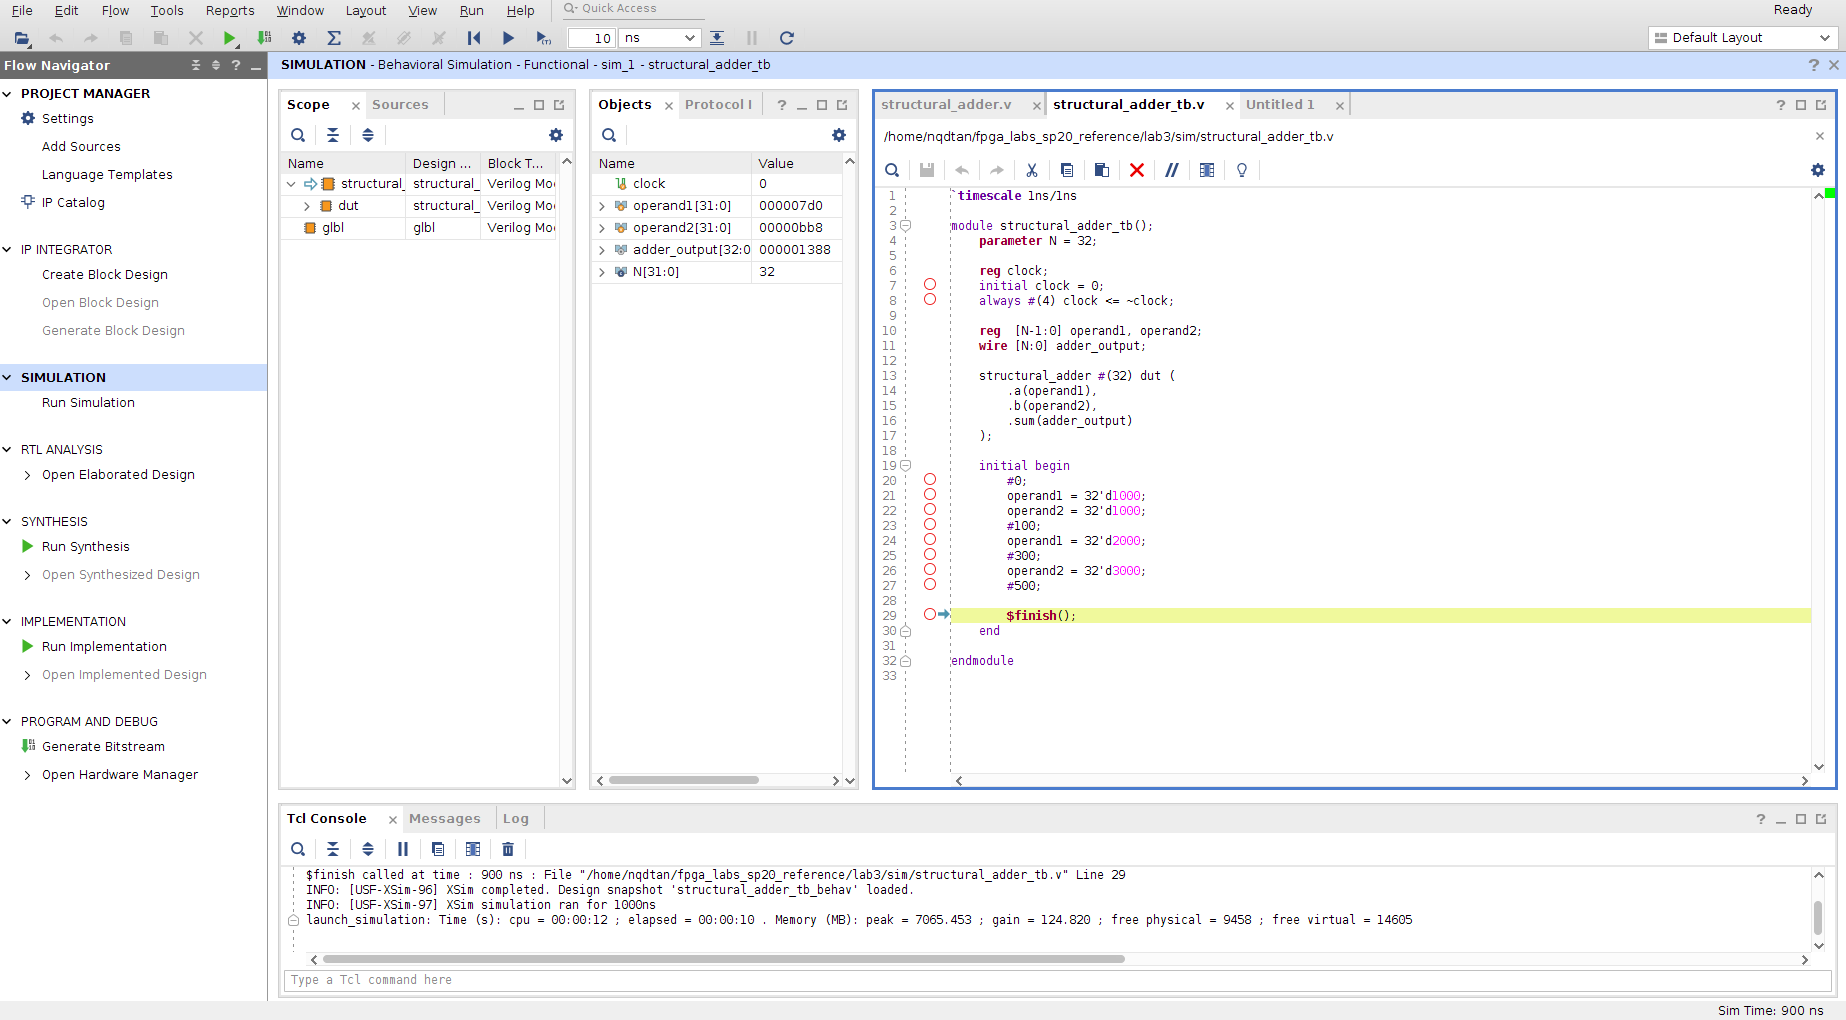
\includegraphics[width=1.0\textwidth]{figs/vivado_sim0.png}
\end{center}

Go to the waveform tab (\emph{Untitled 1}) to observe the waveform. Check the timings of those assignments as well as the values of \verb|adder_output| signal to see if they make sense to you. The simulation should stop at 900ns. By default, the multi-bit signals such as \verb|operand1|, \verb|operand2|, \verb|adder_output| are displayed in hex format. You can convert them to decimal format by selecting those signals, then right click $\rightarrow$ \emph{Radix} $\rightarrow$ \emph{Unsigned Decimal}. You should expect to see something as follows.

\begin{center}
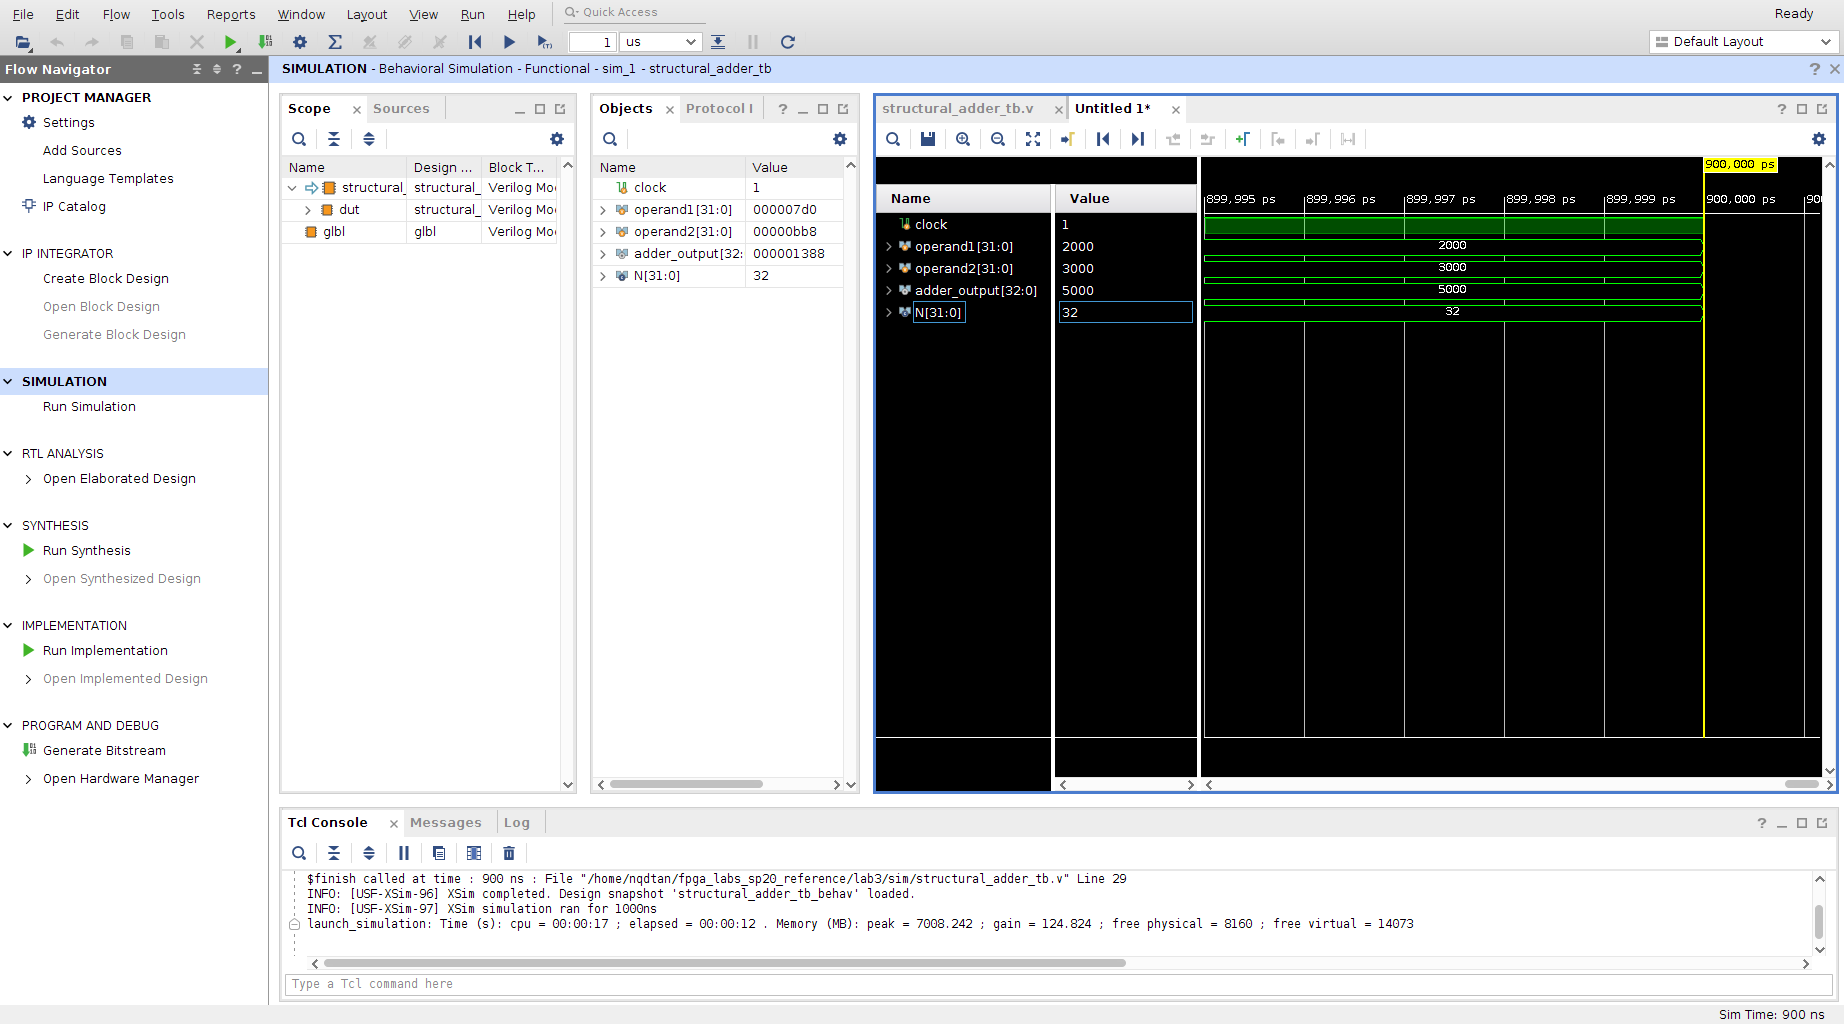
\includegraphics[width=1.0\textwidth]{figs/vivado_sim2.png}
\end{center}

Spend some time to explore the functions of the buttons in the waveform window. Things like \emph{Next Transition} or \emph{Previous Transition} along with \emph{Markers} are helpful when you want to track the transitions of your signals. You can do \texttt{Ctrl + } your mouse wheel to zoom in/out part of the waveform. Click \emph{Zoom Fit} to see the entire waveform from the start to the end.
 
 \begin{center}

\includegraphics[width=0.7\textwidth]{figs/vivado_sim3.png}
\end{center}

Next, we explore the functions of the simulation buttons (right under Vivado top menu bar). Click \emph{Restart} button (or \texttt{Ctrl + Shift + F5}) to restart your simulation. You will see that all the signals are in 'X' state (uninitialized). Click \emph{Run All} button (or \texttt{F3}) to run the simulation. This will run the simulation until finish. The tool also provides an option to run the simulation for some amount of time that you want (click \emph{Run for ...} or \texttt{Shift + F2}). There's also a debug breakpoint capability which we won't cover here.

\begin{center}
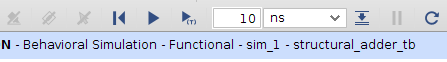
\includegraphics[width=0.4\textwidth]{figs/vivado_sim4.png}
\end{center}

Try changing a few things in the initial block of your testbench. After making changes to the code, you can relaunch the simulation by clicking the \emph{Relaunch simulation} button.

Please note, sometimes Vivado simulator may stop before it actually reaches the \verb|$finish();| statement in your testbench. That's because by default the tool only runs the simulation for a certain duration (which you can change), so don't be confused. In this situation, you can click the \emph{Run All} ("Play") button (or press \texttt{F3}) to continue. Another thing to observe is the progress bar ("Current time") at the bottom of the Vivado program when running simulation. If your simulation runs for a while and does not appear to terminate as you wish, you should stop it, otherwise the program will continues dumping the simulated data to disk and your system may run out of space! A good practice when creating a testbench is to have some code that checks for timeout to abort the simulation. You will see some examples of that in the next section of the lab when we cover the Input Conditioning circuits.

You can also save your waveform (\texttt{Ctrl + S}) before exiting Simulation or Vivado to retain the configuration (such as Decimal radix) for next time you open it up.

\subsection{Questions}\label{sec:Q2}
\begin{enumerate}
  \item The adder output is updated immediately with the inputs. This is because our adder circuit is a combinational circuit. Modify the structural adder so that the adder output is updated at every clock edge. Remember to use a REGISTER module from the EECS151.v library. Don't forget to add it to your project! Run the simulation again to see if your \verb|adder_output| signal now is synchronous with the clock signal (remember to also wire the clock signal to your DUT). Screenshot the waveform and submit it to the lab report (pick a region of the waveform which the output transition w.r.t clock signal can be observed clearly).
  \item Instead of manually setting the values of \verb|operand1| and \verb|operand2| in the initial block, modify the testbench to provide a test vector of 10 values for each of the operands (\verb|operand1| and \verb|operand2|). You can define arbitrary values for your test vectors. A test vector can be an array of wires or regs (or integer) with pre-defined values. Drive each value in the test vectors to your DUT per clock cycle. You can write some sequential always block(s) for this task. Submit the modified testbench and a screenshot of your waveform to the lab report.

Here is an \textit{example} of creating a 2D array of \emph{reg} (works for \emph{wires} too):

\begin{minted}[tabsize=4]{verilog}
reg [7:0] arr [3:0]; // 4 X 8-bit array
arr[0]; // First byte from arr (8 bits)
arr[1][2]; // Third bit of 2nd byte from arr (1 bit)
\end{minted}

\end{enumerate}

Note that you can also have multiple \verb|initial| blocks in your testbench code. The initial blocks run concurrently.

If you are unsure or confused about any of the steps above, don't hesitate to discuss with a TA.

\section{Additional Testbench Techniques}

\begin{itemize}
\item \verb|@(posedge <signal>)| and \verb|@(negedge <signal>)| - These are a different type of delay statement from what you have seen before. \verb|#10| would advance the simulation by 10 timesteps. These commands will advance the simulation until the \verb|<signal>| rises or falls.

For example:
\begin{minted}[frame=single]{verilog}
@(posedge signal);
@(posedge signal);
\end{minted}

Simulation time will advance until we have seen two rising edges of \verb|signal|.

\item \verb|repeat| - it acts like a \verb|for| loop but without an increment variable

For example:
\begin{minted}[frame=single, tabsize=4]{verilog}
repeat (2) @(negedge clk);
repeat (10) begin
  @(posedge clk);
end
\end{minted}

The simulation will advance until we have seen 2 falling clock edges and will then advance further until we have seen 10 rising clock edges.

\item \verb|$display| - acts as a print statement. Similar to languages like C, if you want to print out a wire, reg, integer, etc... value in your testbench, you will need to format the string. It works like \verb|printf()| in C. It is a great debug method if you are not a fan of waveform.

For example:
\begin{minted}[frame=single]{verilog}
$display("Wire x in decimal is %d", x);
$display("Wire x in binary is %b", x);
// You can even print out the current simulation time
$display("Time %d", $time);
\end{minted}

\item \verb|tasks| - tasks are subroutines where you can group and organize some commands rather than haphazardly putting them everywhere. They can take inputs and assign outputs.

\begin{minted}[frame=single, tabsize=4]{verilog}
task wait_for_n_clocks();
input [7:0] num_edges;
begin
  repeat (num_edges) @(posedge clk);
end
endtask
\end{minted}

\item \verb|fork/join| - Allows you to execute testbench code in parallel. You create a fork block with the keyword \verb|fork| and end the block with the keyword \verb|join|.

For example:
\begin{minted}[frame=single, tabsize=4]{verilog}
fork
  begin
    task1();
  end
  begin
    $display("Another thread");
    task2();
  end
join
\end{minted}

Multiple threads of execution are created by putting multiple begin/end blocks in the fork-join block.
In this example, thread 1 runs \verb|task1()|, while thread 2 first \verb|$display|s some text then runs \verb|task2()|.
The threads operate in parallel.

\item Hierarchical Paths - you can access signals inside an instantiated module for debugging purposes. This can be helpful in some cases where you want to look at an internal signal but don't want to create another output port just for debug.

For example:
\begin{minted}[frame=single, breaklines]{verilog}
$display("counter2_val: %d", dut.counter2_val);
$display("counter2_reg_q: %d", dut.counter2_reg.q);
\end{minted}
\end{itemize}

As a general tip, you don't have to create separate projects for different Vivado simulations. You can add all the source files and testbench files to a single project. You need to set which one is the top-level module for \emph{Simulation}. In the \emph{Sources} pane, under \emph{Simulation Sources}, right click on the testbench file of the DUT you want to test and choose \emph{Set as top}.

\section{Input Conditioning Circuits}
To safely use the button signals on the PYNQ board with respect to clock signal of our circuits, we have to design the input conditioning circuits to handle metastability and button bounce. Check the prelab reading on Debouncer circuit \ref{sec:begin} if you have not done so.

\subsection{Synchronizer}
In Verilog (RTL), digital signals are either 0's or 1's.
In a digital circuit, a 0 or 1 corresponds to a low or high voltage.
If the circuit is well designed and timed (fully synchronous), we only have to worry about the low and high voltage states.

The signals coming from the push buttons and slide switches on the PYNQ board don't have an associated clock (asynchronous).
When the button signals are put through a register, its hold or setup time may be violated.
This may put that register into a \textit{metastable} state (Figure \ref{fig:metastability}).

\begin{figure}
  \centerline{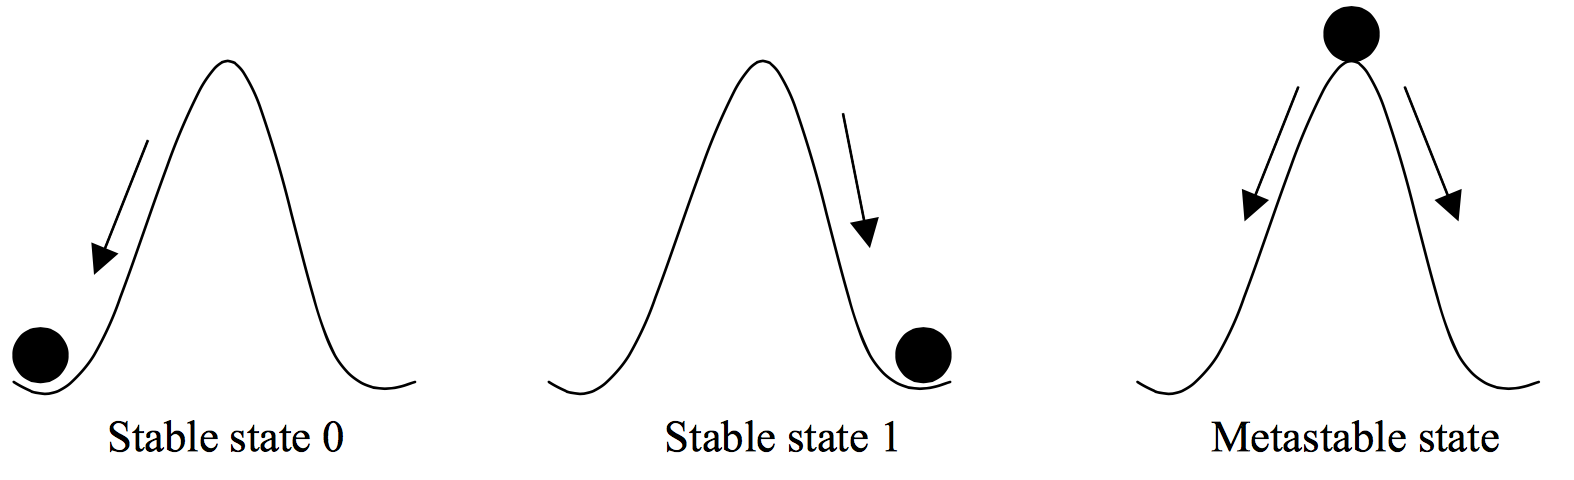
\includegraphics[height=3cm]{figs/metastability.png}}
  \caption{The `ball on a hill' metaphor for metastability. If a register's timing constraints are violated, its output voltage oscillates and after some time unpredictably settles to a stable state.}
  \label{fig:metastability}
\end{figure}

%In a fully synchronous circuit, the timing tools will determine the fastest clock frequency under which the setup time constraints are all respected and the routing tools will ensure that any hold time constraints are handled.
An asynchronous signal could violate timing constraints, and cause a `mid-rail' voltage from a register to propagate to other logic elements.
This can cause catastrophic timing violations that the tools never saw coming.

We will implement a synchronizer circuit that will safely bring an asynchronous signal into a synchronous circuit.
The synchronizer needs to have a very small probability of allowing metastability to propagate into our synchronous circuit.

This synchronizer circuit for this lab is relatively simple (Figure \ref{fig:synchronizer}).
For synchronizing one bit, it is a pair of flip-flops connected serially.

\begin{figure}[H]
  \vspace{0.5cm}
  \centerline{\includegraphics[width=0.4\textwidth]{figs/synchronizer.png}}
  \caption{1-bit 2 Flip-Flop Synchronizer}
  \label{fig:synchronizer}
\end{figure}

Edit \verb|lab2/src/synchronizer.v| to implement the two flip-flop synchronizer.
This module is parameterized by a \verb|width| parameter which controls the number of one-bit signals to synchronize.

\subsubsection{Synchronizer Simulation}
A testbench is provided in \verb|lab2/sim/sync_tb.v|. Run it using Vivado simulation.

\subsection{Debouncer}
\begin{figure}[H]
  \centerline{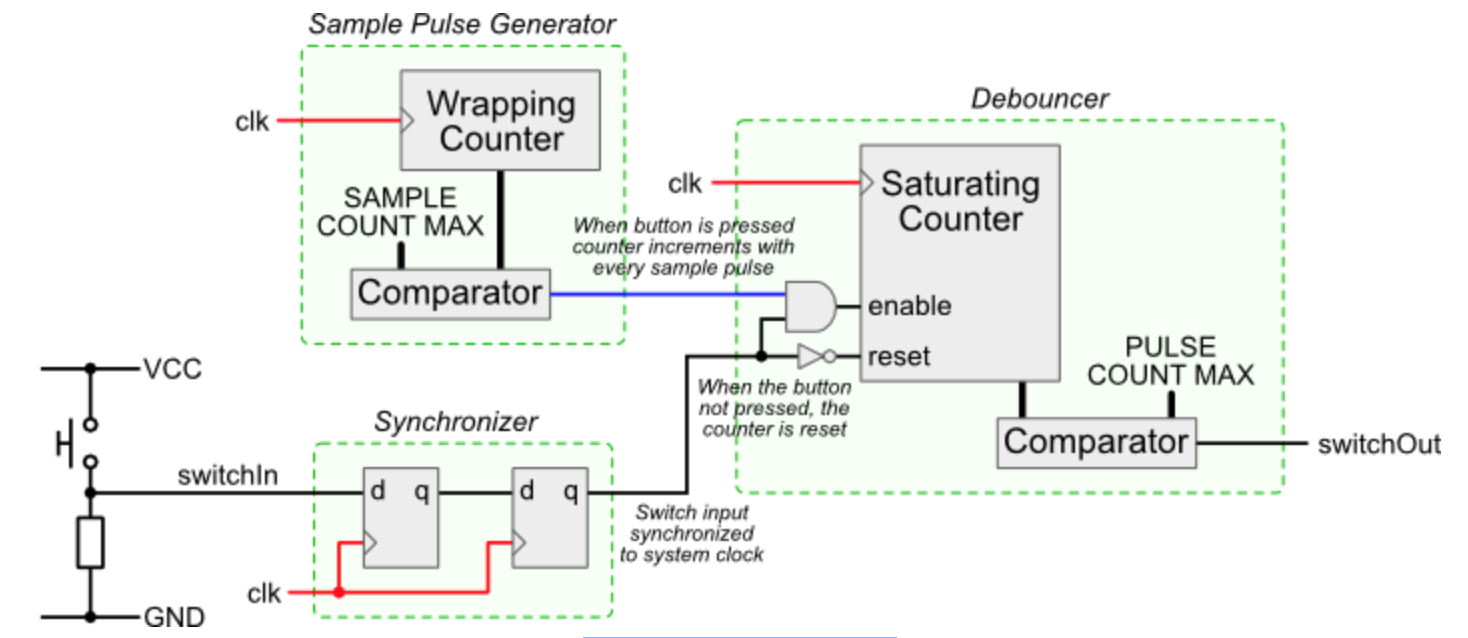
\includegraphics[height=5cm]{figs/debouncer.png}}
\end{figure}

Recall this graphic from the prelab debouncer reading.

The debouncer circuit takes a button's glitchy digital signal and outputs a clean signal indicating a single button press.
The reason we need a circuit for this can be seen in the figure below.

\begin{figure}[H]
  \centerline{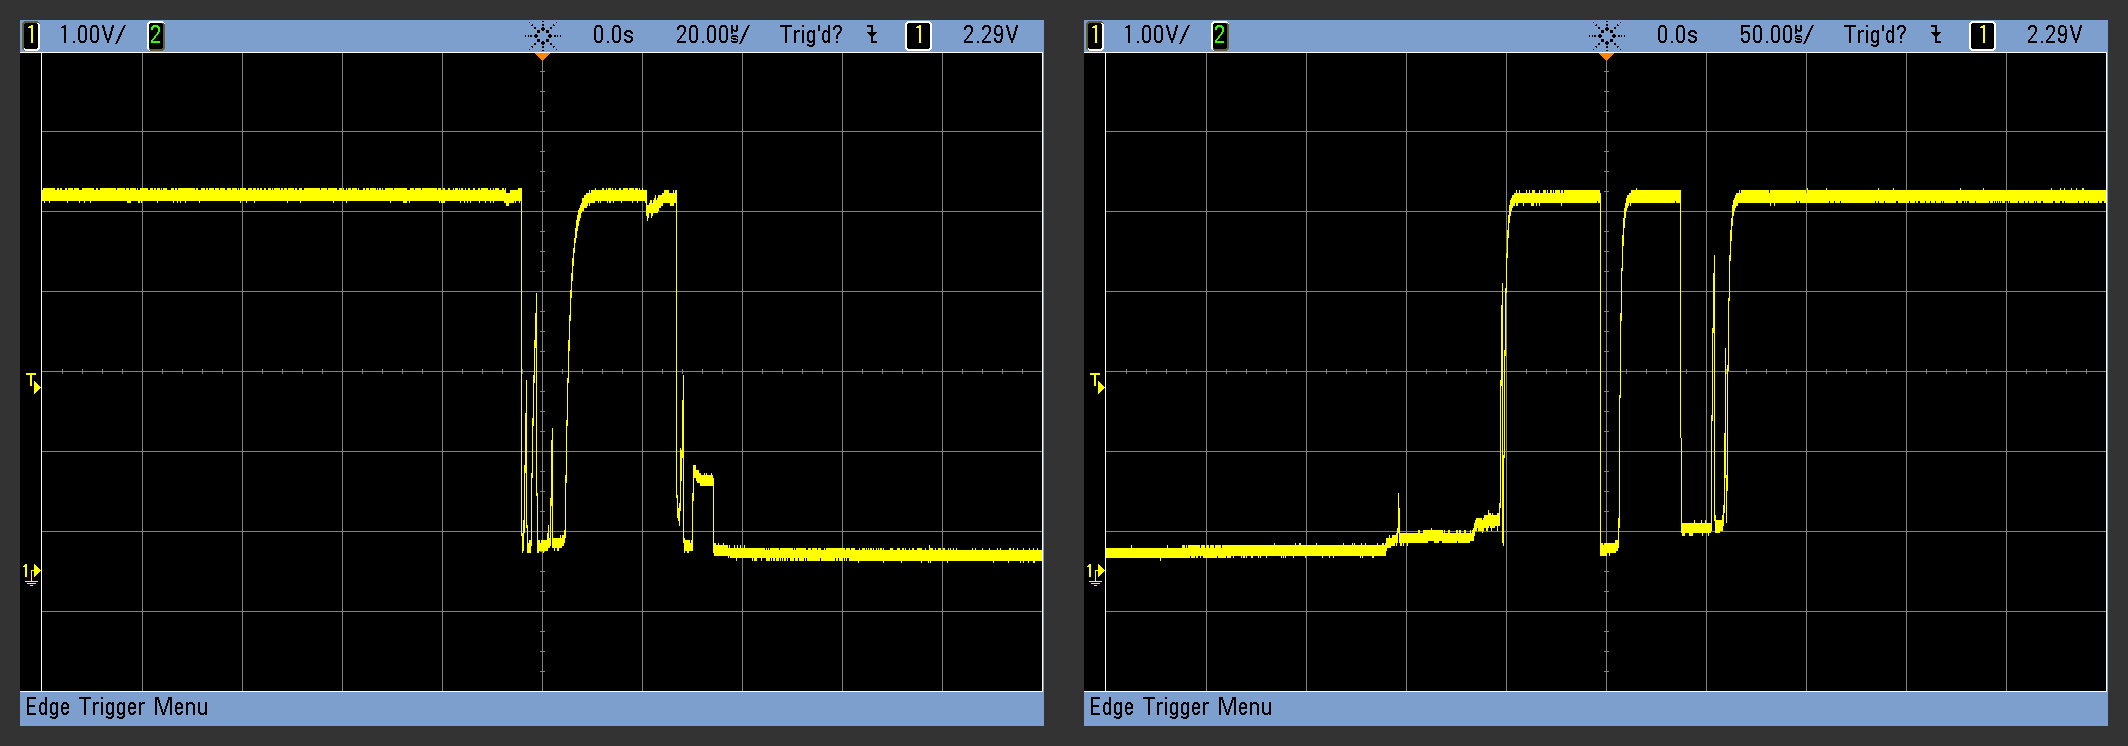
\includegraphics[width=0.5\textwidth]{figs/bouncing.png}}
\end{figure}

When we press or depress a button, the signal doesn't behave like a perfect step function.
Instead the button signal is glitchy due to mechanical ``bounce''.
If we naively used the button signal directly there would be many spurious ``button presses".

Look at \verb|lab2/src/debouncer.v|.
This is a parameterized debouncer which can debounce \verb|width| signals at a time.
The other parameters reference the constants used in the circuit from the prelab reading.

The debouncer consists of:
\begin{enumerate}
  \item \textbf{Sample Pulse Generator} - Tells our saturating counter when to sample the input signal. It should output a 1, every \verb|SAMPLE_CNT_MAX| clock cycles. By default \verb|SAMPLE_CNT_MAX| is set to 25000.
  \item \textbf{Saturating Counter} - This is a counter that counts up to \verb|PULSE_CNT_MAX|.
    If the sample pulse is high at a clock edge, increment the counter if the input signal is also high, else reset the counter to 0.
    Once the saturating counter reaches \verb|PULSE_CNT_MAX|, it should hold that value indefinitely until the sampled input signal becomes 0.
    The \verb|debounced_signal| of your debouncer should be an equality check between the saturating counter and \verb|PULSE_CNT_MAX|.
\end{enumerate}

You can use the same sample pulse generator for all input signals into your \verb|debouncer|, but you should have a separate saturating counter per input signal.

\subsubsection{Debouncer Simulation}
A testbench has been provided in \verb|lab2/sim/debouncer_tb.v|. Make sure you understand what the testbench is doing. Run it as usual.

The debouncer testbench has 2 tests:
\begin{enumerate}
  \item Verifies that if a glitchy signal initially bounces and then stays high for \textbf{less} than the saturation time, that the debouncer output never goes high.
  \item Verifies that if a glitchy signal initially bounces and then stays high for \textbf{more} than the saturation time, that the debouncer goes high and stays high until the glitchy signal goes low.
\end{enumerate}

Pay attention to the printouts in the \emph{TCL Console} to see if tests are passed or failed.

\subsection{Edge Detector}
The debouncer will act to \emph{smooth-out} the button press signal.
It is then followed up with an edge detector that can take the low-to-high transition of the debouncer output and use it to generate a 1 clock cycle wide pulse that the rest of our digital design can use.

Create a parameterized-width edge detector in \verb|lab2/src/edge_detector.v|.

\subsubsection{Edge Detector Simulation}
A testbench is provided in \verb|edge_detector_testbench.v|. Run as usual.

The edge detector testbench tests 2 scenarios, when the \verb|signal_in[0]| transitions from low-to-high, and so does \verb|signal_in[1]| a few cycles after. At each time, the corresponding bit of \verb|edge_detect_pulse| goes high at the next clock edge and stays high for one cycle.

\subsection{Button Parser on the FPGA}
Now that we have tested all the modules required to produce a clean, stable button press signal. It's time to put everything together. In this section, we design a counter that uses the buttons on the PYNQ board to provide some functionalities.

\subsubsection{Counter with with Button Parser}
Look at \verb|src/button_parser.v| which combines the synchronizer, debouncer, and edge detector in a chain.
Create a Vivado project (or reuse existing project). Add these files

\verb|lab2/src/synchronizer.v|, \verb|lab2/src/debouncer.v|, \verb|lab2/src/edge_detector.v|,

\verb|lab2/src/button_parser.v|, \verb|lab2/src/z1top_mode_counter.v|, \verb|lib/EECS151.v|,

and \verb|lab2/constraints/pynq-z1.xdc|. Set \verb|z1top_mode_counter| as the top-level module. Generate a bitstream and test this circuit on the PYNQ board. Check that each button performs the right action as written in \texttt{z1top\_mode\_counter.v}.

\subsubsection{Play and Pause your Counter}

Right now, your \texttt{z1top\_mode\_counter.v} is in a static mode; you can only increment or decrement the counter value for each button press. Modify the code such that when you press BTN2, your counter starts incrementing every one second (running mode), and pauses when you press BTN2 again (static mode). It is up to you if you may or may not want to update your counter with BTN0 or BTN1 when your counter is in running mode.

We'd like suggest that you think about the structure of your design ahead of coding. The debouncer circuit figure above is a great example. Remember that Verilog coding is all about describing your hardware circuit! Sketch a block diagram of your mode counter circuit in terms of the \texttt{button\_parser} block and some register blocks from \verb|lib/EECS151.v| as you see fit. Label the relevant input and output signals. Feel free to use any logic gates, MUXes, or adders. Don't worry about listing all the details. Submit your sketched diagram in your report.

\section{Lab Deliverables}
\subsection{Lab Checkoff (due: 11.00AM, Feb 10th, 2020)}
To checkoff for this lab, have these things ready to show the TA:
\begin{enumerate}
  \item Demonstrate a working mode counter with button parser. Show that you can toggle the modes of your counter with BTN2.
\end{enumerate}

\subsection{Lab Report (due: 11.59PM, Feb 10th, 2020)}\label{sec:labreport}

Please submit a short report to Gradescope with the following items.

\begin{enumerate}
  \item Your answers to the questions \ref{sec:Q1} and \ref{sec:Q2}. In addition, please also submit the block diagram of your mode counter.
\end{enumerate}

\appendix
\section{Local Dev Setup}

Besides Vivado, we'll cover installing free tools for simulation for each OS here so
you can have more options to do your lab/homework exercises.

\subsection{Linux/OSX}
\begin{enumerate}
  \item Add vivado to your \verb|$PATH| by adding this in your \verb|.bashrc|:

    \verb|export PATH="/opt/Xilinx/Vivado/2019.1/bin:$PATH"|
  \item Install Icarus Verilog
    \begin{itemize}
      \item Linux: \verb|sudo apt install iverilog|
      \item OSX: \verb|brew install icarus-verilog|
    \end{itemize}

  \item Install Verilator
    \begin{itemize}
      \item Linux: \verb|sudo apt install verilator|
    \end{itemize}

  \item Install gtkwave
    \begin{itemize}
      \item Linux: \verb|sudo apt install gtkwave|
      \item OSX: \href{https://sourceforge.net/projects/gtkwave/files/gtkwave-3.3.100-osx-app/gtkwave.zip/download}{\color{blue}{Download the app}}
    \end{itemize}
\end{enumerate}

In a terminal you should be able to successfully run \verb|vivado|, \verb|iverilog|, \verb|gtkwave|.

\subsection{Windows}
Windows packages for \href{http://bleyer.org/icarus/}{\color{blue}{Icarus are available}}. You should be able to download the appropriate .exe for your machine. Gtkwave can be installed along with Icarus (just make sure you check the box for it). Lastly, here is a link to install \href{https://www.cygwin.com/install.html}{\color{blue}{Cygwin}}. When you install Cygwin, you need to check the boxes for make and git as shown in Fig. \ref{fig:cygwin}, and also Python 3.6.

\begin{figure}[ht]
  \centering
  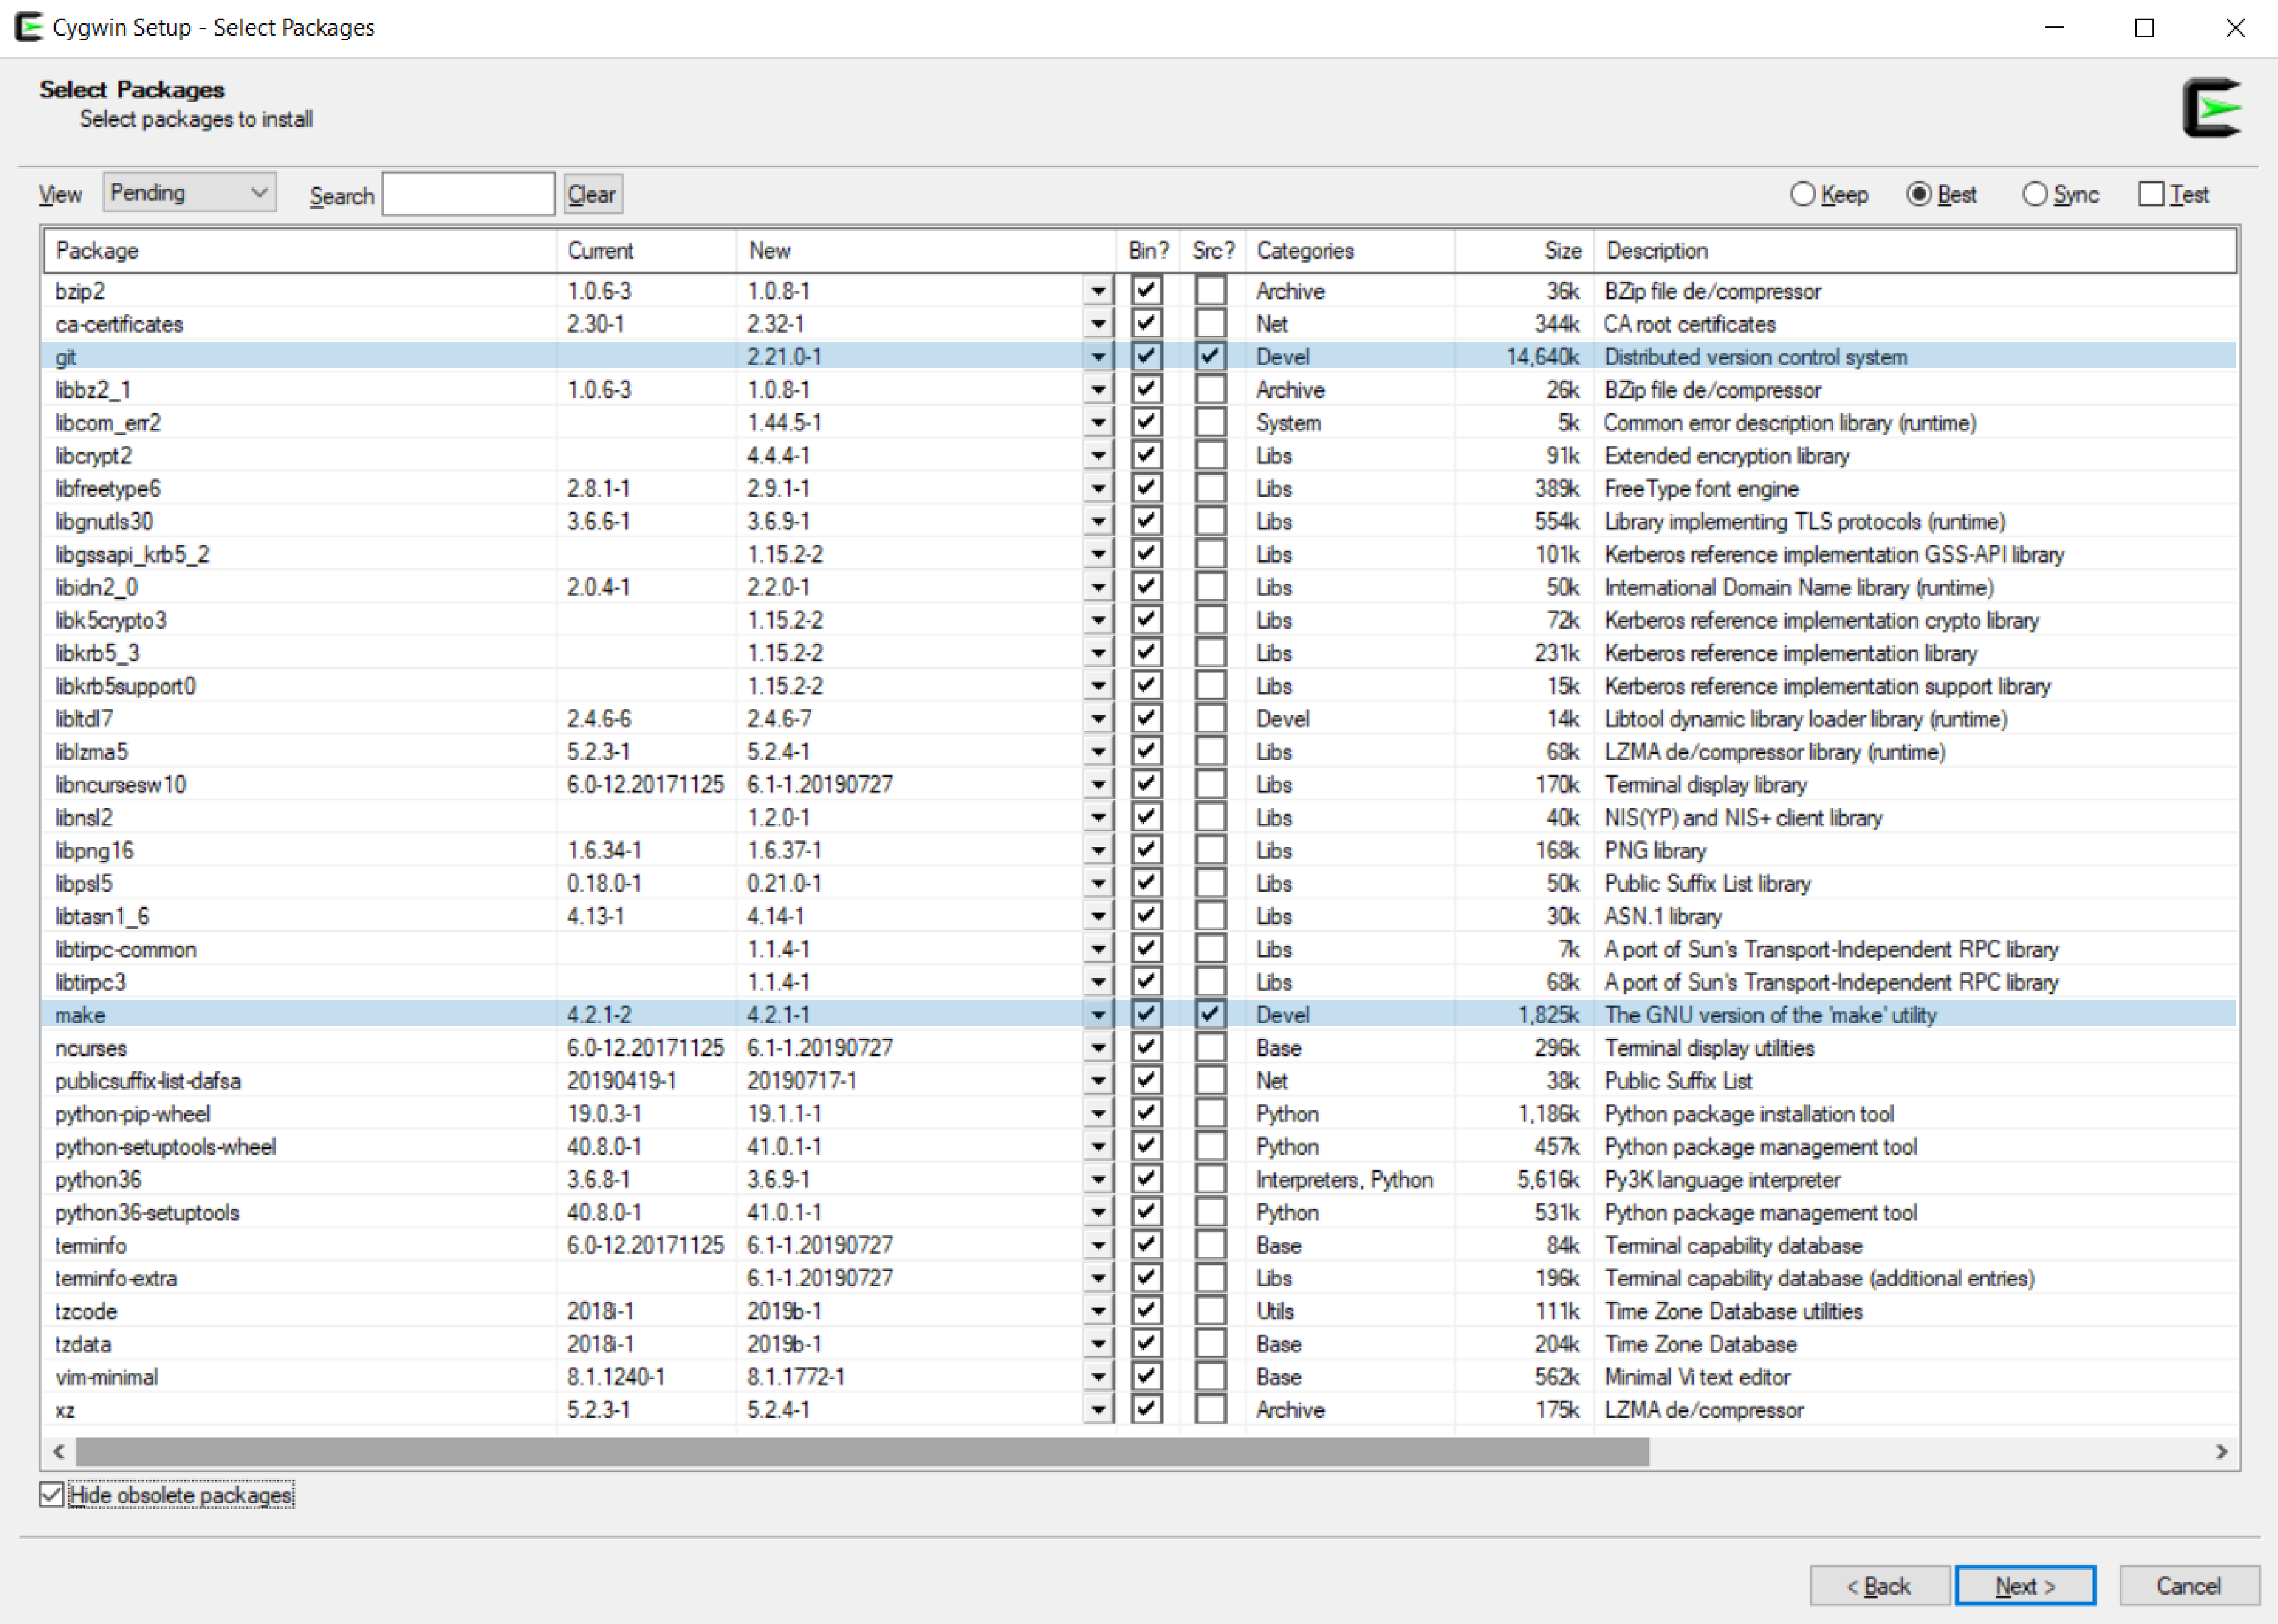
\includegraphics[width=0.5\textwidth]{figs/cygwin_install.png}
  \caption{Check make and git with your cygwin install!}
  \label{fig:cygwin}
\end{figure}

After installing Icarus, gtkwave, and cygwin, you'll need add Vivado, Icarus, and gtkwave to your Windows PATH with the below steps.
\begin{itemize}
    \item Go the windows control panel and find the "Edit the system variables menu". Alternatively, if you just search for "system variables", the menu should pop up.
    \item Click the "Environment Variables" button near the window's bottom right corner (Fig. \ref{fig:envVars1}).
    \item Double click the "Path" variable in the user variables dialog  (Fig. \ref{fig:envVars2}).
    \item Click the next empty row and paste the path of the appropriate program  (Fig. \ref{fig:envVars3}). Hit okay and you're done!
\end{itemize}

\begin{figure}[H]
  \centering
  \begin{minipage}{0.5\textwidth}
    \centering
    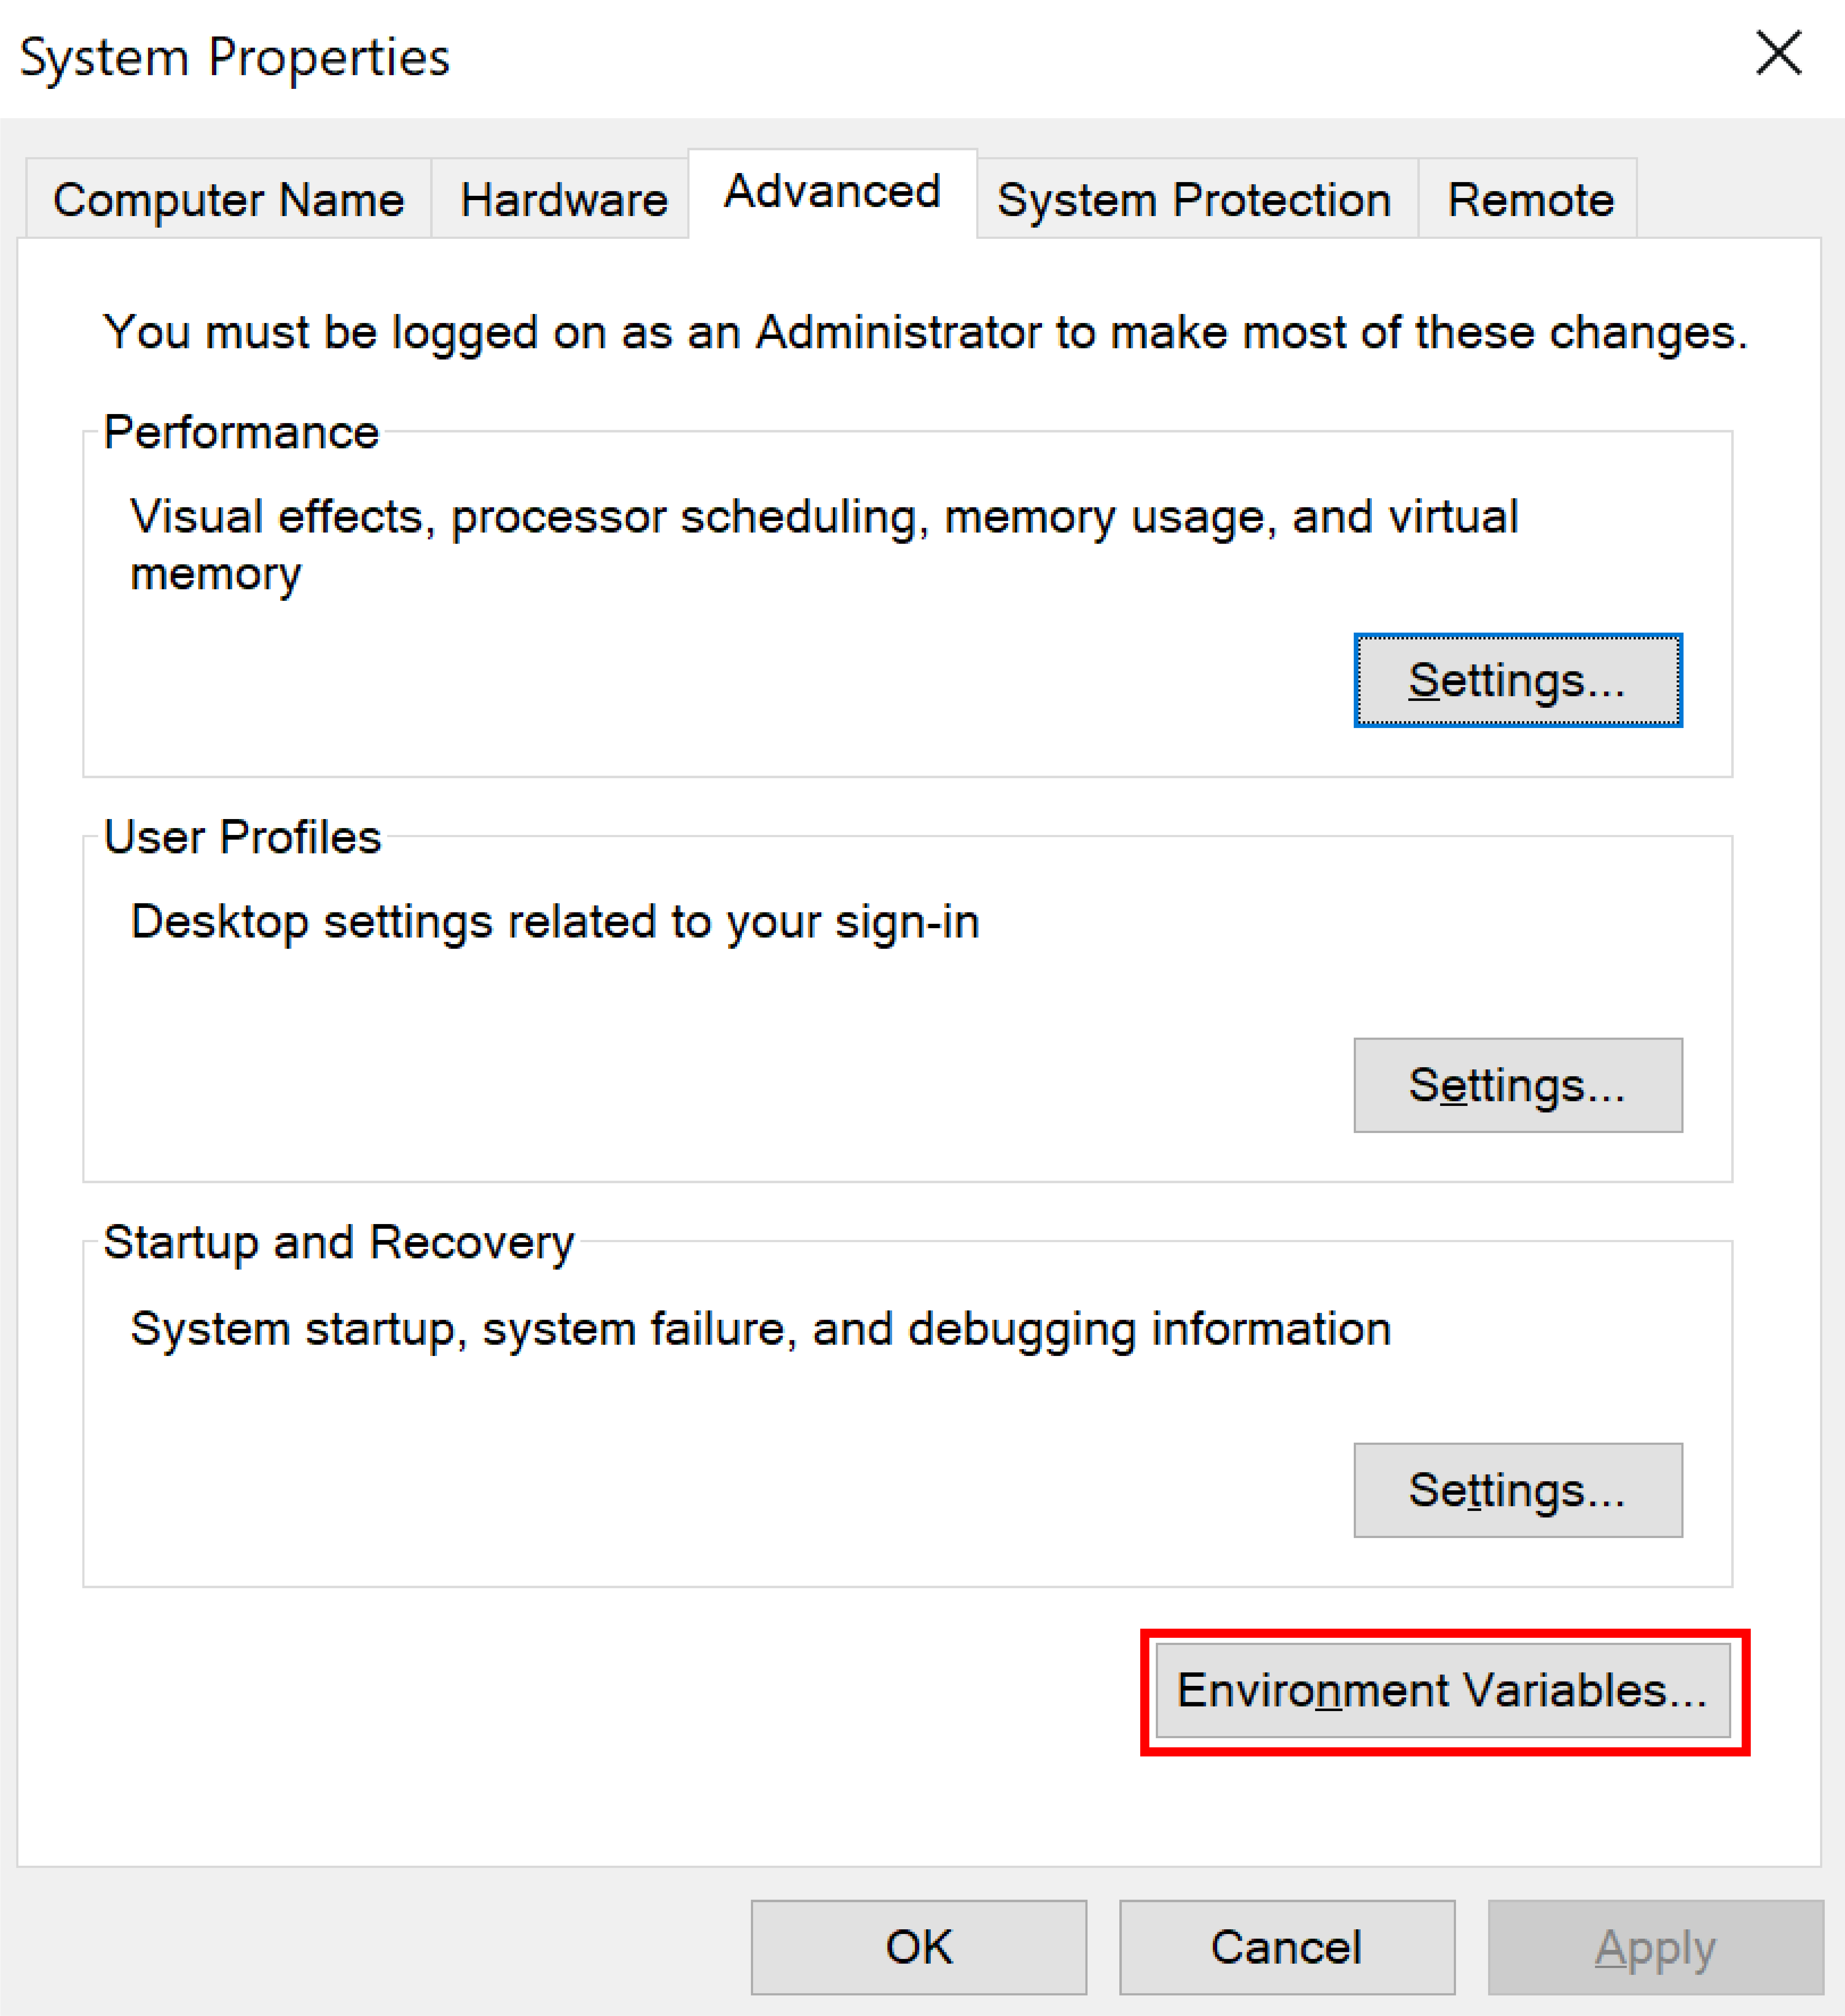
\includegraphics[width=0.5\textwidth]{figs/environment_variables_1a.png}
    \caption{The System variables dialogue.}
    \label{fig:envVars1}
  \end{minipage}\hfill
  \begin{minipage}{0.5\textwidth}
    \centering
    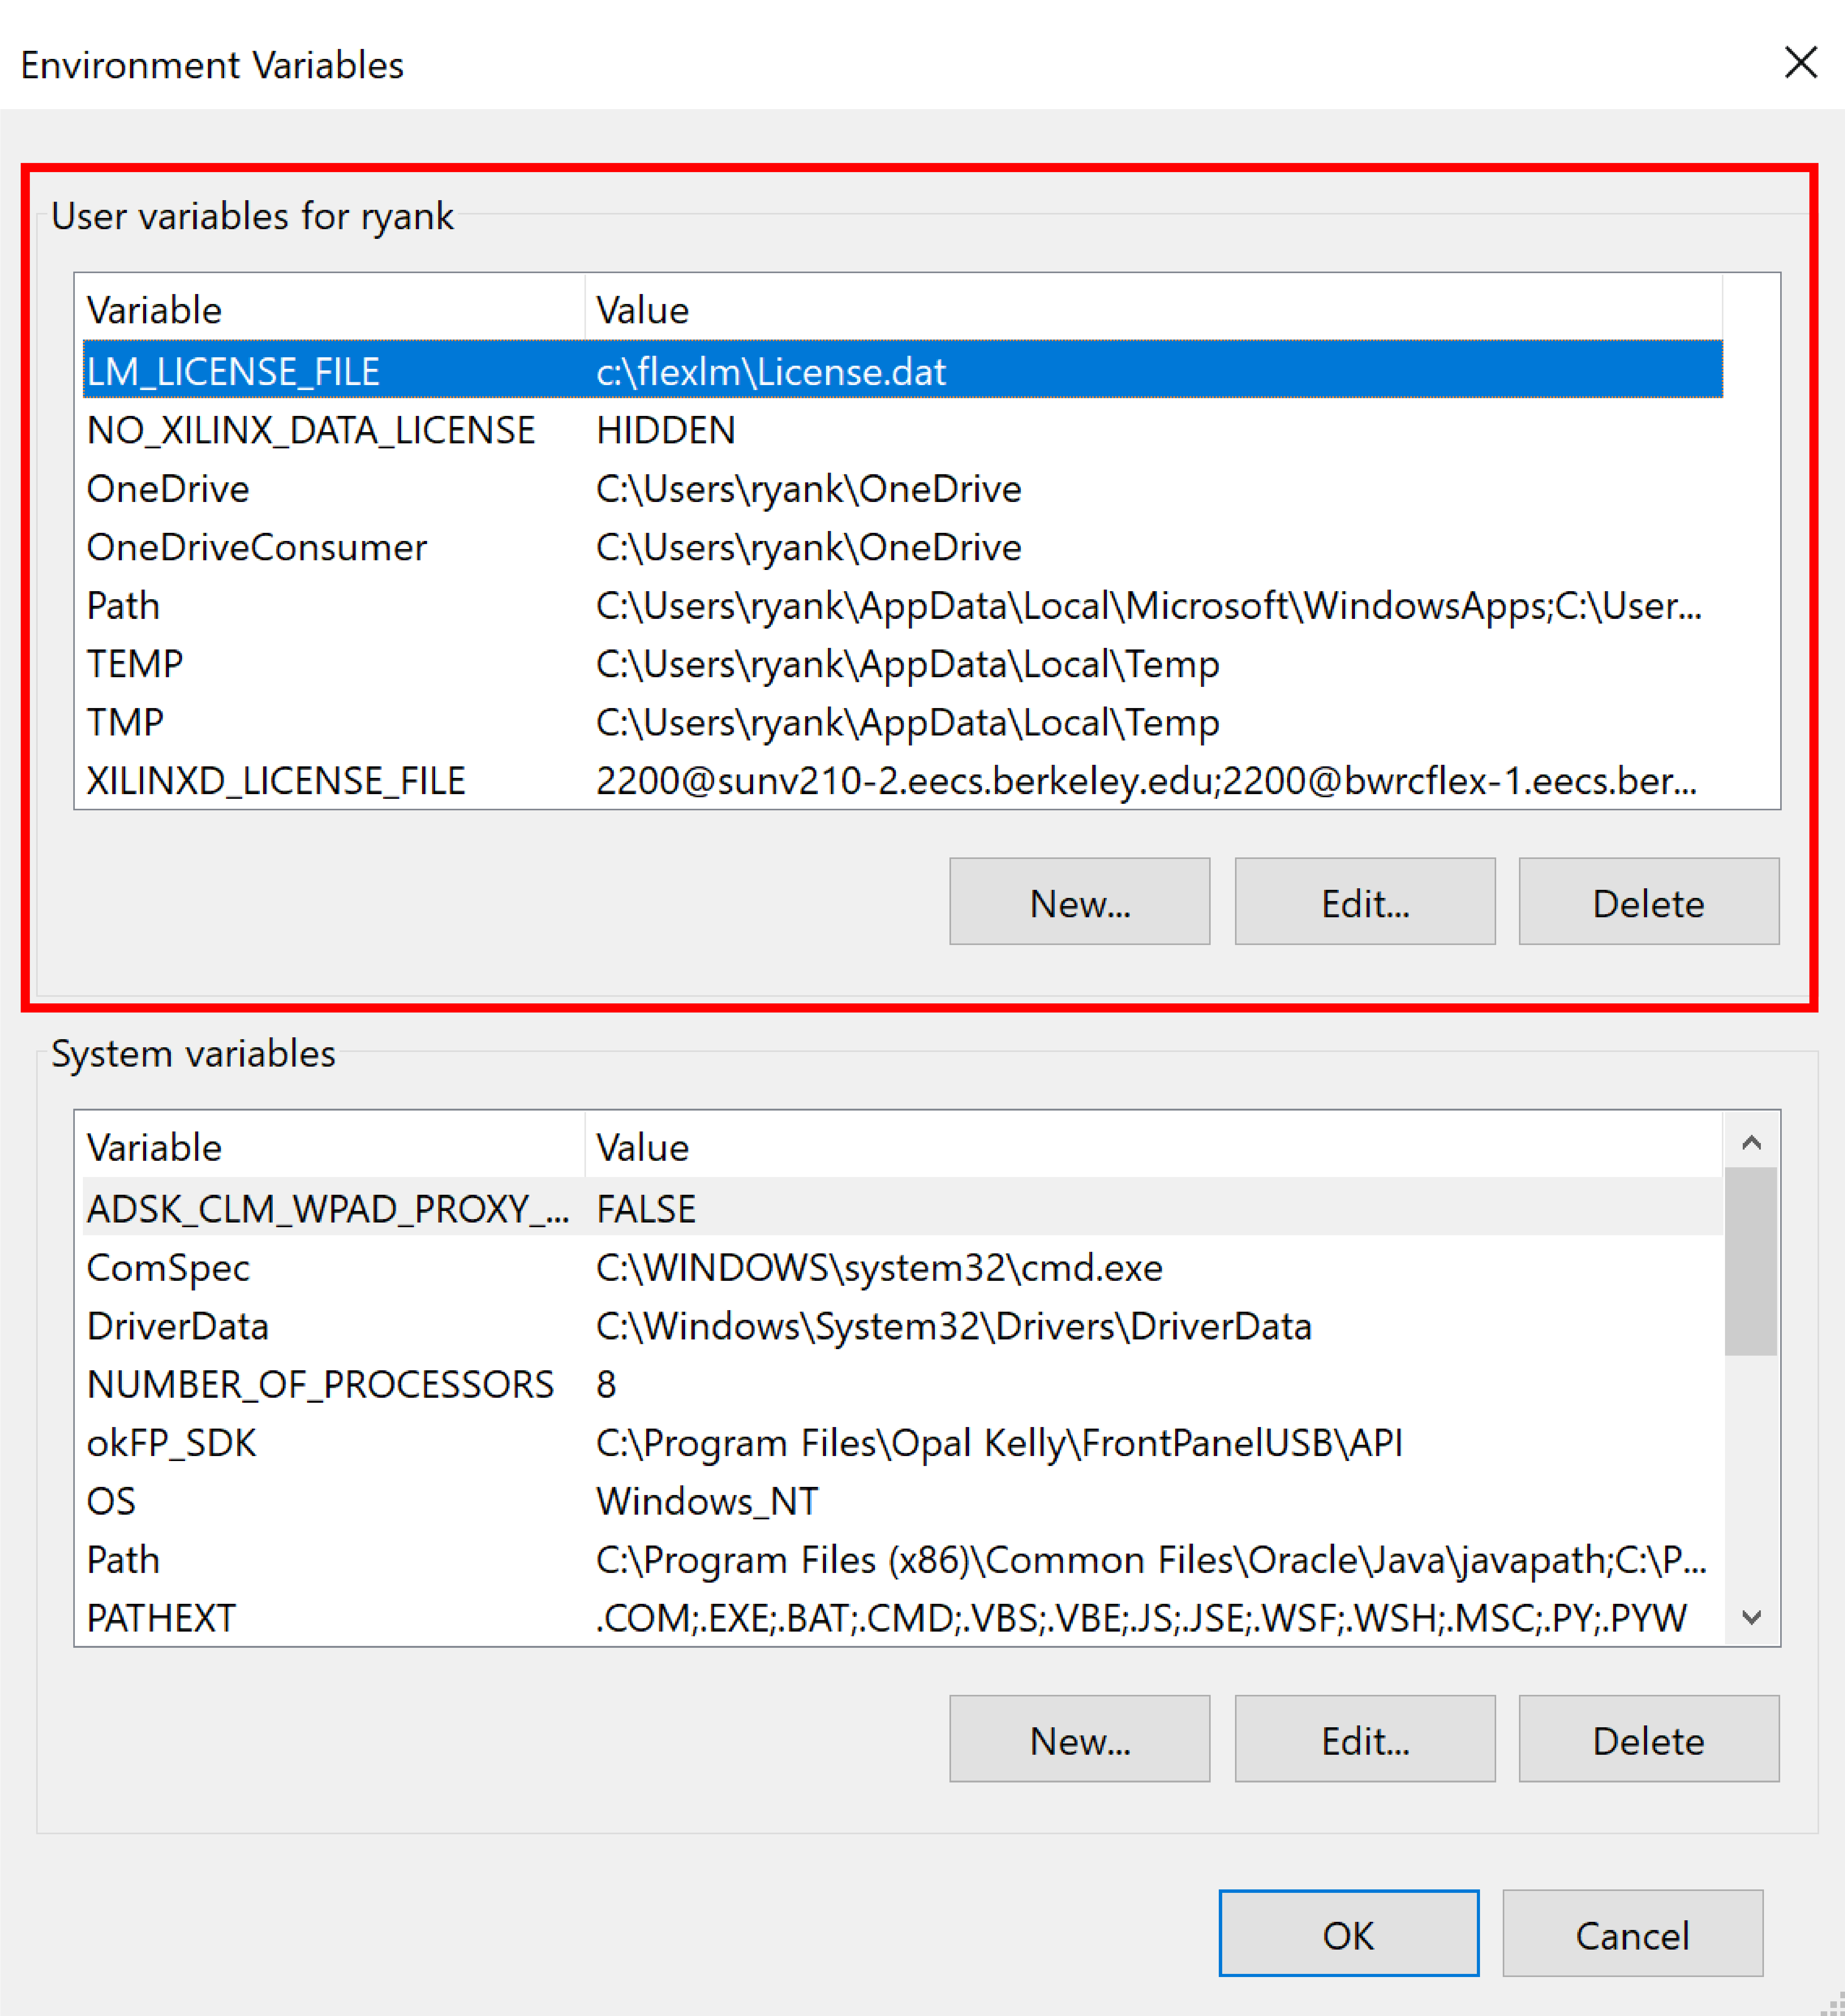
\includegraphics[width=0.5\textwidth]{figs/environment_variables_2a.png}
    \caption{Environment variables dialogue.}
    \label{fig:envVars2}
  \end{minipage}
\end{figure}

\begin{figure}[ht]
  \centering
  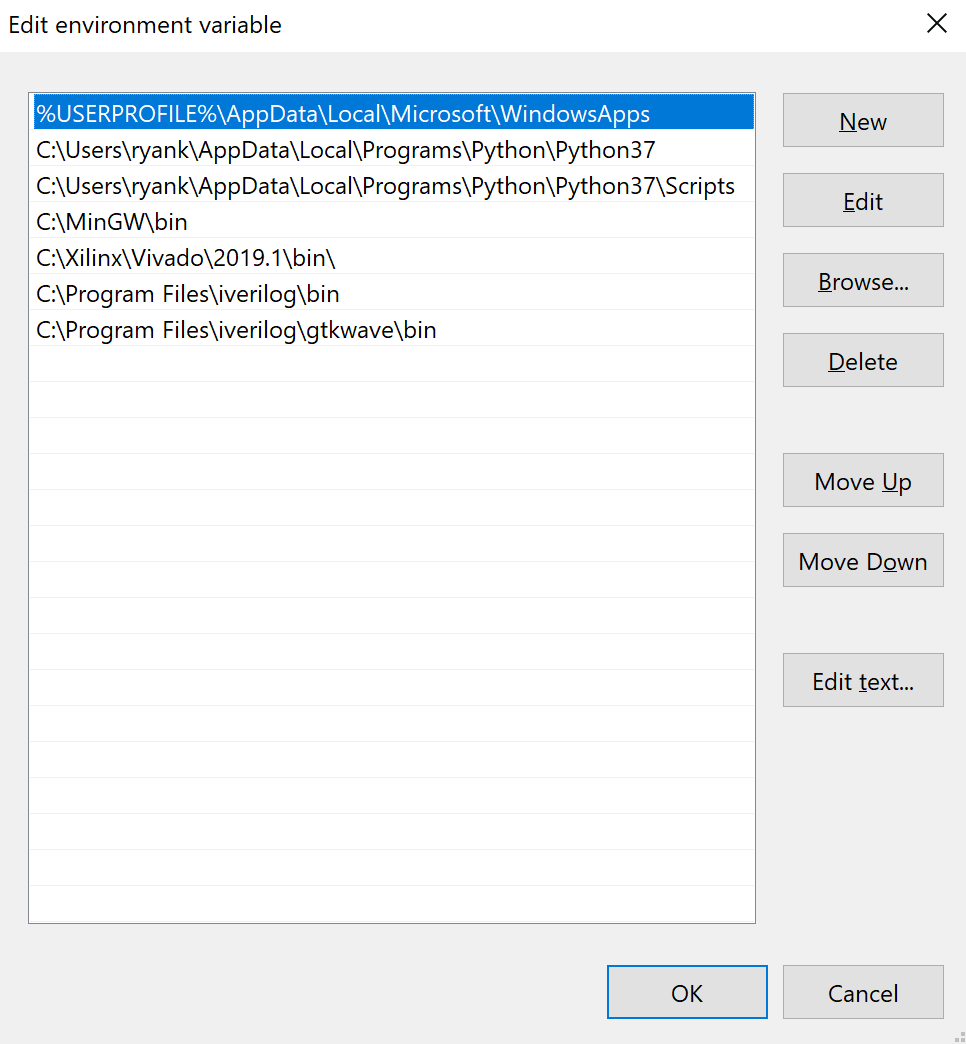
\includegraphics[width=0.5\textwidth]{figs/environment_variables_3.png}
  \caption{Adding programs to your PATH.}
  \label{fig:envVars3}
\end{figure}
\newpage
\section*{Ackowlegement}
This lab is the result of the work of many EECS151/251 GSIs over the years including:
\begin{itemize}
\item Sp12: James Parker, Daiwei Li, Shaoyi Cheng
\item Sp13: Shaoyi Cheng, Vincent Lee
\item Fa14: Simon Scott, Ian Juch
\item Fa15: James Martin
\item Fa16: Vighnesh Iyer
\item Fa17: George Alexandrov, Vighnesh Iyer, Nathan Narevsky
\item Sp18: Arya Reais-Parsi, Taehwan Kim
\item Fa18: Ali Moin, George Alexandrov, Andy Zhou
\item Sp19: Christopher Yarp, Arya Reais-Parsi
\item Fa19: Cem Yalcin, Rebekah Zhao, Ryan Kaveh, Vighnesh Iyer
\item Sp20: Tan Nguyen
\item Fa20: Charles Hong, Kareem Ahmad, Zhenghan Lin
\end{itemize}

\end{document}
